\section{Beyond the Scanchain}
\label{sec:beyond_scanchain}
The biggest limitation of the Tiny Tapeout architecture was the IO latency.
For Tiny Tapeout 4 a new architecture was needed, and a series of proposals was gathered from the community.
An online video call was held and the 10 proposals discussed.
The winning design was a fairly straightforward multiplexer design.

\begin{figure}[htp]
\centering
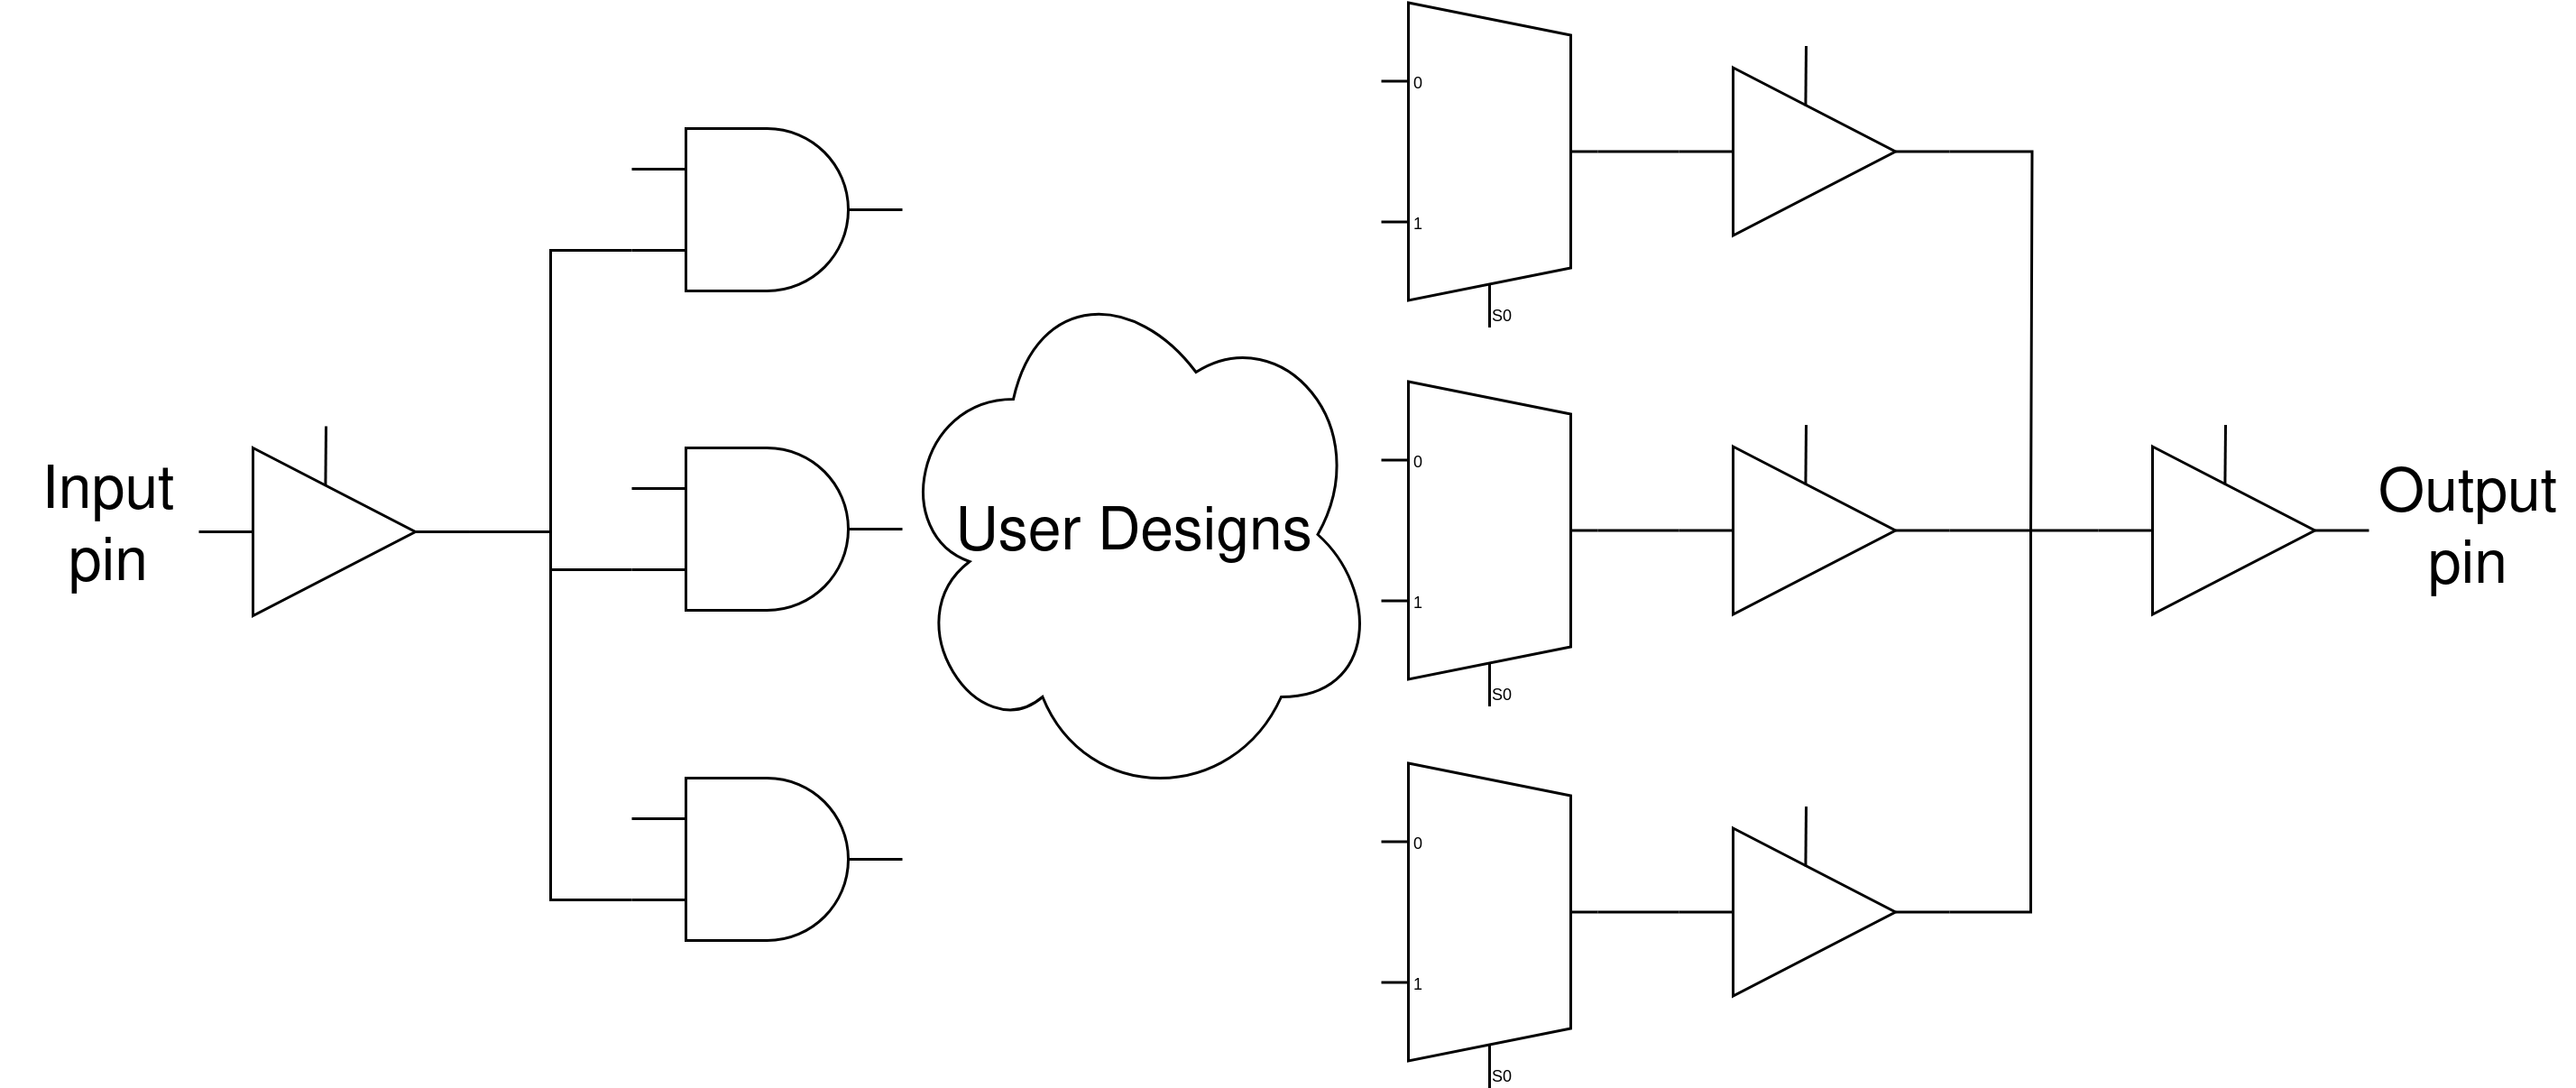
\includegraphics[width=\columnwidth]{./Figs/mux architecture.png}
\caption{The multiplexer design.}
\label{fig:multiplexer_design}
\end{figure}

The physical layout consists of a central controller connected up and down to two vertical spines.
Twenty-four horizontal muxes connect to the spine with each supporting 16 designs.
This allows up to 384 separate single tile designs.
Multiple tile designs were also enabled, allowing a maximum project size of \(2 \times 8\) tiles or \(1359 \times 225 \mu m\) - around 20,000 logic cells.

\begin{figure}[htp]
\centering
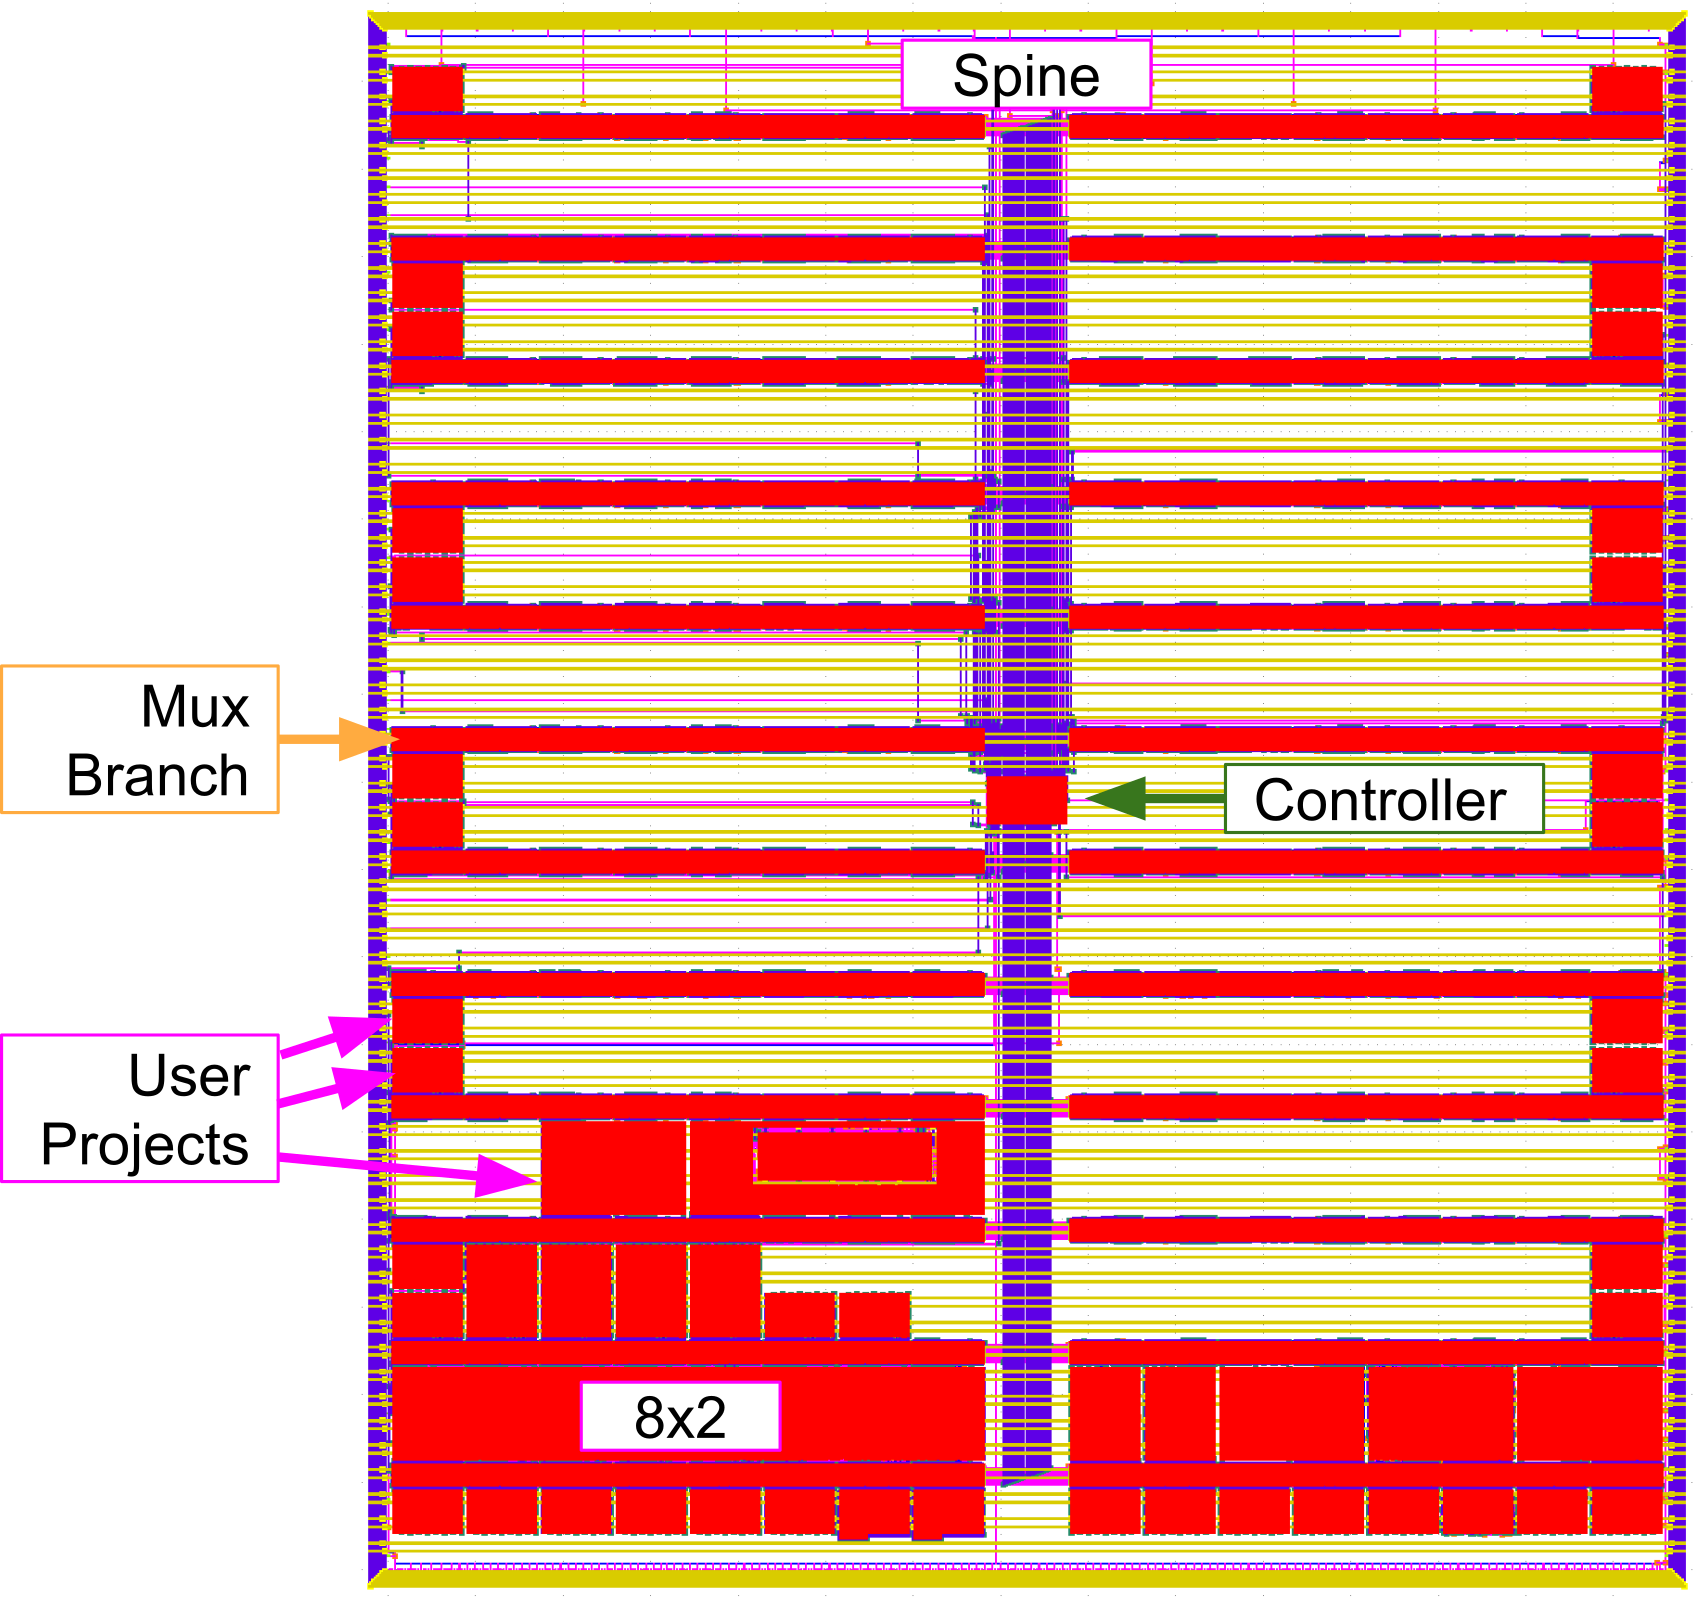
\includegraphics[width=\columnwidth]{./Figs/tt3p5 layout.png}
\caption{The TT03.5 test design.}
\label{fig:TT03_5_test_design}
\end{figure}

Another major limitation of TT1 to 3 was the small number of IO.
The scan controller used 9 GPIOs to select the currently active design, which, while simplifying the demo board, wasted valuable pins.
With TT04, the parallel design selection was dropped in favor of a serial protocol.
The extra pins were then used as bidirectional pins, giving each design clock, reset, and 24 IO.

\begin{table}[htp]
\centering
\caption{Comparison between TT03 and TT04}
\label{tab:comparison_TT03_TT04}
\begin{tabular}{@{}lcc@{}}
\toprule
Parameters & Tiny Tapeout 3 & Tiny Tapeout 4 \\
\midrule
Max clock speed & \(12.5 kHz\) & \(50 MHz\) \\
Max design size & \(150 \times 170 \mu m\) & \(1359 \times 225 \mu m\) \\
Input pins & \(8\) & \(10\) \\
Output pins & \(8\) & \(8\) \\
Bidirectional I/O pins & None & \(8\) \\
Custom GDS file & \xmark & \checkmark \\
\bottomrule
\end{tabular}
\end{table}

An invite-only experimental shuttle~\cite{tinytapeout03p5} was submitted with 32 designs to Efabless chipIgnite 2306C.
Two of the designs included a power gate as a stepping stone to supporting analog and mixed-signal designs.
